\chapter{Задача сегментации и виды разметки данных} \label{chapt1}


\section{Постановка заачи.Сильная и слабая разметка данных}
Центральным объектом рассмотрения в данной работе является задача сегментации медицинских изображениях.
При решении задачи {\bf сегментации}  новообразований/поражений/аномалий необходимо для каждого пикселя изображения установить его принадлежность к проблемной области(положительному классу) на снимке. При этом каждый набор изображений может поставляться с некоторого рода дополнительными сведениями, называемыми {\bf разметкой}.

Говорят, что набор изображений $\{M_i\}_{i\in I}\subset \mathcal{M}^{mxn}$ имеет {\bf сильную разметку}, если для каждого пикселя с координатами $(x,y)$ известно, относится ли он к положительному классу или нет. При этом каждому изображению $M_i$ ставится в соответствие битовая маска $B_i$, отражающая данную информацию: $$\{B_i\}_{i\in I} \subset \mathcal{M}^{mxn},$$ где $$\forall i \in I,  \forall x,y: 1\le x \le m, 1\le y \le n, B_i(x,y) \in \{0,1\}.$$

Получение сильной разметки данных в ручном режиме сопряжено со значительными временными и финансовыми затратами: попиксельная разметка изображений в высоком разрешении требует кропотливого труда высококлассного опытного специалиста, а также клинического подтверждения диагноза, к примеру, путём взятия биопсии. Для оценки можно принять, что разметка одного изображения занимает около 5 минут. Тогда разметка 10.000 изображений вручную потребует 50.000 минут или более 100 рабочих дней непрерывного труда без учёта времени на валидацию разметки. В таких условиях целесообразно каким-то образом устранить необходимость наличия сильной разметки. Однако возникает вопрос: информации какого типа окажется достаточно для получения сходной по качеству системы сегментации с той, которая получена на основе набора данных с сильной разметкой. Наборы изображений, для которых отсутствует сильная разметка, но имеется иная разметка данных, позволяющая каким-то образом установить наличие либо отсутствие пикселей положительного класса, называются {\bf слабо размеченными}. Примерами слабой разметки может служить:

\begin{itemize}
    \item Наличие классификации(прямое отнесение изображения к одному из двух классов в зависимости от наличия новообразований);
    \item Наличие размеров новообразований если таковые имеются на изображении;
    \item Приблизительная локализация локализация: точка и радиус диаметра окружности около неё;
    \item Наличие прямоугольной рамки, заключающей новообразование(Bounding box);
    \item $\dots$
\end{itemize}

В данной работе речь пойдёт главным образом о первых двух видах слабой разметки.

В следующем разделе приведём несколько примеров задач сегментации изображений, возникающих в медицинской практике.

\section{Примеры задач сегментации}

\subsection{Гистопатология}

{\bf Задача:} по данным высококачественным изображениям тканей распознать наличие поражений, локализовать их и разбить на кластеры(\ref{fig:histo}).
\\
{\bf Пример работы:} \cite{xu_weakly_2014}


\begin{figure}[ht] 
  \center
  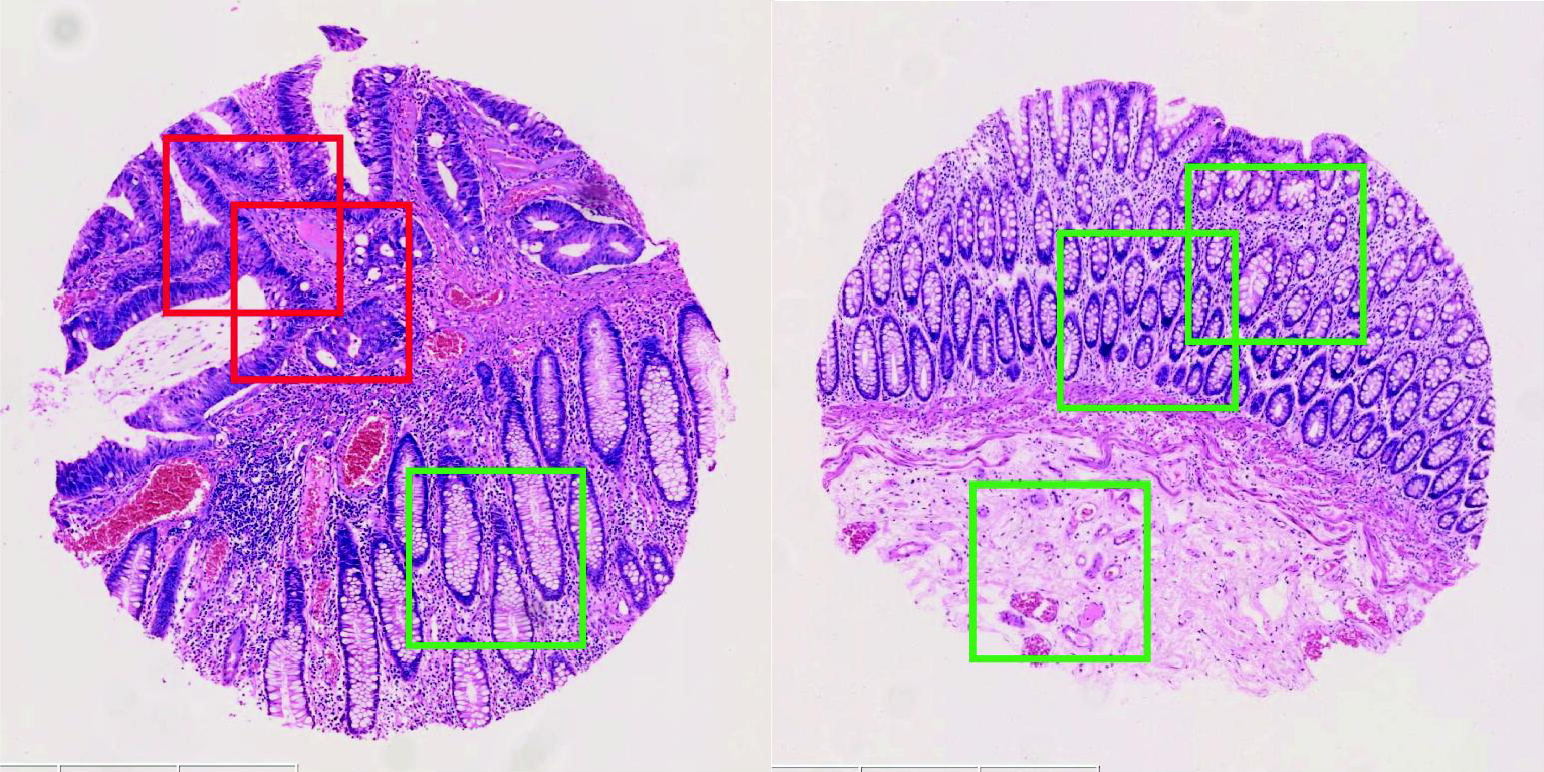
\includegraphics [scale=0.27] {images/histo_1.png}
  \caption{Примеры здоровых(зелёные) и поражённых(красные) раком областей ткани; \cite{xu_weakly_2014}} 
  \label{fig:histo}  
\end{figure}



\subsection{Задачи, связанные с изображениями мозга}

\subsubsection{Выделение белого вещества в мозге}
{\bf Задача:} по данным изображениям МРТ сегментировать участки, представляющие собой белое вещество мозга(\ref{fig:whitematter});
\\
{\bf Пример работы:} \cite{white_matter}


\begin{figure}[ht] 
  \center
  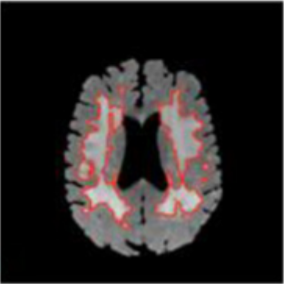
\includegraphics [scale=1.0] {images/white_matter.png}
  \caption{ Пример изображения с сегментацией белого вещества\cite{white_matter} } 
  \label{fig:whitematter}  
\end{figure}


\subsubsection{Сегментация опухолей головного мозга}

{\bf Задача:} детектировать и локализовать злокачественные новообразования (\ref{fig:brats}).

{\bf Пример работы}: \cite{BRATS_winning_2018}
\begin{figure}[ht] 
  \center
  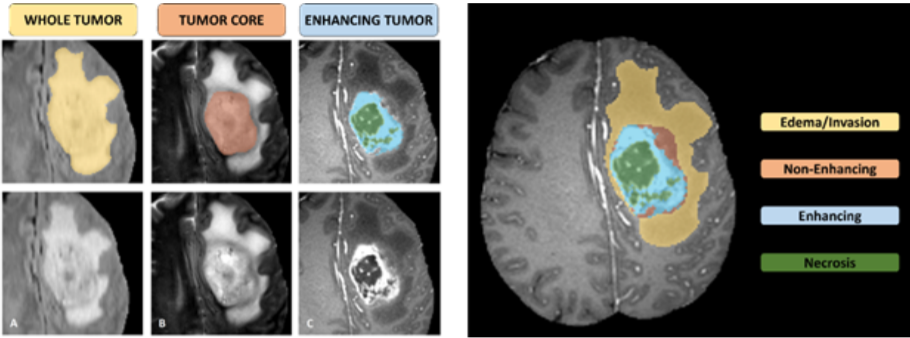
\includegraphics [scale=0.8] {images/brats.png}
  \caption{ Пример изображения мозга с сегментацией новообразования и его составных частей \cite{BRATS_2018} } 
  \label{fig:brats}  
\end{figure}


\subsection{Задачи, связанные с раком молочной железы}

\subsubsection{Сегментация тканей молочной железы}
{\bf Задача:} отделить на снимке более плотные ткани от мягких. Более плотные ткани связаны с повышенным риском развития злокачественных новообразований, однако средняя плотность тканей не является постоянной для всех пациентов(на это влияет в том числе процент жировой ткани), что усложняет задачу выделения плотных областей на снимке(\ref{fig:breast_1r}, \ref{fig:breast_2})
\\
{\bf Пример работы:} \cite{breast_tissue}


\begin{figure}[h] 
  \center
  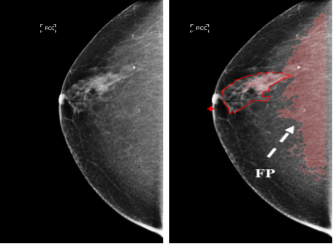
\includegraphics [scale=1.0] {images/breast_1.png}
  \caption{ Пример сегментации(красная сплошная линия) для пациента с низкой совокупной плотностью тканей\cite{breast_tissue}} 
  \label{fig:breast_1r}  
\end{figure}

\begin{figure}[!htb] 
  \center
  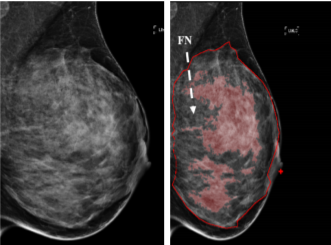
\includegraphics [scale=1.0] {images/breast_2.png}
  \caption{ Пример сегментации(красная сплошная линия) для пациента с высокой совокупной плотностью тканей\cite{breast_tissue}} 
  \label{fig:breast_2}  
\end{figure}
\
\subsubsection{Сегментация злокачественных новообразований}

{\bf Задача:} детектировать и локализовать злокачественные новообразования.\ref{fig:breast_3}
\\
{\bf Пример работы:} \cite{zhu_mil}

\begin{figure}[h] 
  \center
  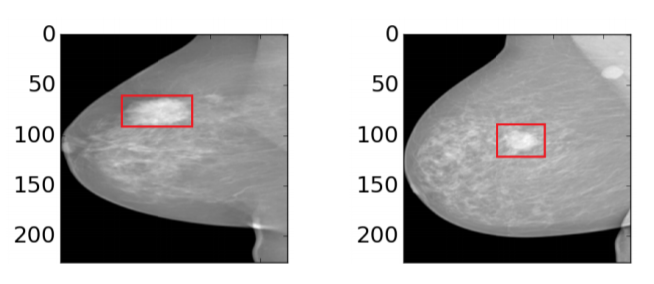
\includegraphics [scale=0.8] {images/breast_cancer.png}
  \caption{ Пример сегментации новообразований в молочной железе\cite{zhu_mil} }
  \label{fig:breast_3}  
\end{figure}



\subsection{Задачи, связанные с раком предстательной железы}

{\bf Задача:} сегментировать предстательную железу на изображении, детектировать и локализовать доброкачественные и  злокачественные новообразования(\ref{fig:prostate}).

{\bf Пример работы}: \cite{prostate-cancer}

\begin{figure}[h] 
  \center
  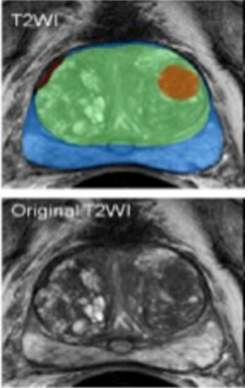
\includegraphics [scale=0.8] {images/prostate.png}
  \caption{ Пример изображения с выделенными {\color{blue} железой}, {\color{green} центральной частью}, {\color{orange} доброкачественным новоообразованием}, {\color{red} злокачественным новоообразованием} \cite{prostate-cancer}} 
  \label{fig:prostate}  
\end{figure}



\subsection{Задачи, связанные с поражениями сетчатки глаза}

{\bf Задача:} на данном изображении сетчатки глаза сегментировать поражения, связанные с диабетичесской ретинопатией.

{\bf Пример работы:}

\begin{figure}[h] 
  \center
  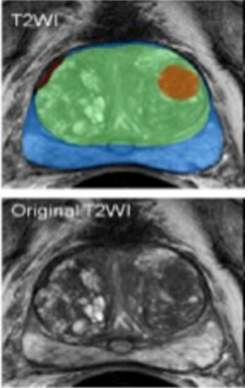
\includegraphics [scale=0.8] {images/prostate.png}
  \caption{ Пример изображения с выделенными {\color{blue} железой}, {\color{green} центральной частью}, {\color{orange} доброкачественным новоообразованием}, {\color{red} злокачественным новоообразованием}} 
  \label{prostate}  
\end{figure}


\section{Данные}

Для разработки системы сегментации нами были использованы данные конкурса BRATS2018. Данный набор данных содержит 285 пациентов с диагнозом глиома. Для каждого пациента предоставлен набор слоёв МРТ в аксиальной проекции. Для каждого слоя дана попиксельная разметка опухоли, если она представлена в данном сечении. Сегментированная опухоль также разделена на несколько составных частей, однако мы в своей работе используем сегментацию опухоли целиком("whole tumor" на изображении ниже \ref{fig:bratss}).  Томографические снимки могут исполняться в различных контрастах. В наших экспериментах был использован контраст T1Gd. 

\begin{figure}[ht] 
  \center
  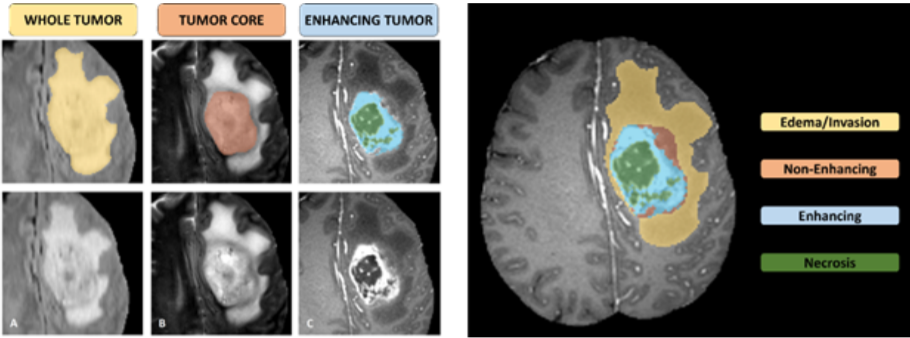
\includegraphics [scale=0.6] {images/brats.png}
  \caption{ Пример изображения мозга с сегментацией новообразования и его составных частей} 
  \label{fig:bratss}  
\end{figure}
Для каждого пациента серия снимков была выровнена таким образом, чтоб минимизировать фоновую площадь изображения(см. \ref{fig:transform}). Затем все изображения были приведены к формату 170x140.

\begin{figure}[ht] 
  \center
  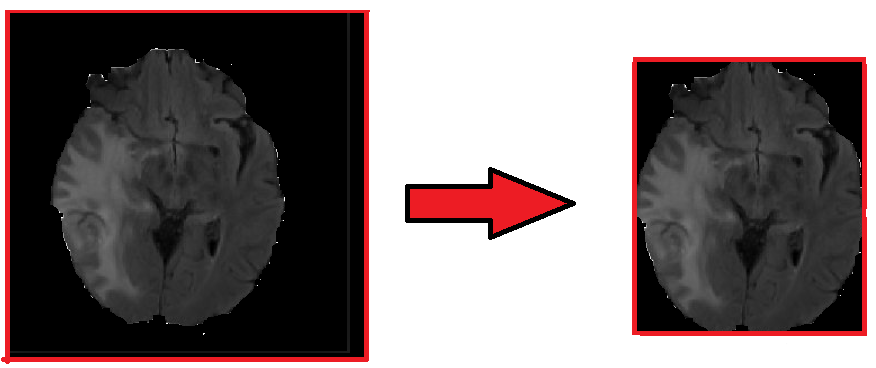
\includegraphics [scale=0.6] {images/transform.png}
  \caption{ Пример выравнивания серии изображений по крайним для нее достижимым границам изображения} 
  \label{fig:transform}  
\end{figure}

С целью упрощения реализации целей и задач данной ранной работы на даннном этапе при выборе слоёв, содержащих опухоль, мы ограничились слоями, в которых опухоль занимает не менее 10\% от площади сечения {\bf мозга}. В дальнейшем также будет обсуждаться переход к более общей задаче.
\section{Метрика}

Для задачи сегментации при обучении на данных с попиксельной разметкой обычно используют два вида метрик:
\begin{itemize}
    \item Индекс сходства Дайса(Dice index);
    \item Перекрестная энтропия(Binary crossentropy);
\end{itemize}

$$\text{Dice~index}(P,T) := \frac{2\sum_{i,j}P_{ij}T_{ij}}{\sum_{i,j}P^2_{i,j} + \sum_{i,j}T^2_{i,j}},$$
где P-пиксельная карта - предсказание($P_{i,j}\in [0,1]$), T - бинарная пиксельная карта($T_{i,j}\in\{0,1\}$). В качестве функции потерь при постановке задачи оптимизации метрики в терминах минимизации используют функцию потерь Дайса(Dice loss):

$$\text{Dice~loss} := 1 - \text{Dice~index}$$

Во избежание возможных проблем с делением на ноль используют параметр сглаживания(smooth), который часто берут равным 1:

$$\text{Dice~index}(P,T) := \frac{2\sum_{i,j}P_{ij}T_{ij} + smooth}{\sum_{i,j}P^2_{i,j} + \sum_{i,j}T^2_{i,j} + smooth},$$

Функция перекрёстной энтропии определяется следующим образом:

$$\text{Binary~crossentropy}(P, T) := -\sum_{i,j}\Large[T_{i,j}\log{P_{i,j}} + (1-T_{i,j})\log{(1-P_{i,j})}\Large]$$

В дальнейшем обе эти метрики будут использованы и сравнены друг с другом с точки зрения результатов сегментации. Преимуществом индекса Дайса перед перекрёстной энтропией является наглядность его геометрической интерпретации: в дискретном виде "удвоенное пересечений двух изображений делится на их суммарную площадь". Приведём примеры изображений, демонстрирующие те или иные значения функции потерь Дайса , 


\section{Результаты}

Согласно <<ref>>, в настоящее время лучшие результаты для сегментации опухоли целиком(whole tumor) составляют порядка {\bf 0.9} в терминах Dice Loss. При этом данные результаты были получены путём обучения на всём наборе данных с использованием сильной разметки. Наши эксперименты, проведённые с такими уже ставишими классическими архитектурами для задачи сегментации, как DenseNet и ResNet-50 в режиме encoder-decoder, успеха не возымели. Прямая оптимизация давала в среднем результаты {\bf худшие 0.3} в терминах Dice Loss, даже принимая во внимание упрощение задачи, допущенное в самом начале. 

Это обстоятельство подтолкнуло нас к поиску менее тривиальной структуры, позволяющей при этом совместное использование данных с сильной и слабой разметкой. В разделе, послвящённом совметсному обучению, можно ознакомиться в том числе и с результатами сегментации,  обученной на сильно размеченных наборах данных.




